\section{Multiple testing}
Recall that when we test a hypothesis $H$, we either claim it is non-significant or reject it. 

We wish to test null hypotheses $H_1, \dotsc, H_m$, of which $m_0$ are true,
and we let $R$ denote the amount of rejected hypotheses. We then define
\begin{table}[H]
	\centering
	\begin{tabular}{c || c | c | c}
		& Claimed non-significant & Rejected & Total\\ \hline \hline
		True hypotheses & $N_{00}$ & $N_{01}$ & $m_0$\\ \hline
		False hypotheses & $N_{10}$ & $N_{11}$ & $m - m_0$ \\ \hline
		Total & $m - R$ & $R$
	\end{tabular}
\end{table}
Note that the $N_{ij}$ are unobserved random variables.

Furthermore, we let $I_0 \subseteq \qty{1, \dotsc, m}$ denote the set of true hypotheses, and we let $p_i$ denote the $p$-value of the individual hypothesis test satisfying
\[
\PP(p_i \leq \alpha) \leq \alpha \qquad\forall \alpha \in [0, 1],
\]
so the chance of rejecting a true null hypothesis at $\alpha$-level is at most $\alpha$. 

\begin{definition}
	The \emph{familywise error rate} or FWER is $\FWER \ceq \PP(N_{01} \geq 1)$, the probability that at least one true hypothesis is rejected. 
\end{definition}

A procedure for testing multiple hypotheses with $\FWER \leq\alpha$ has a chance of at most $\alpha$ to reject at least one true hypothesis. Note that this is a very strong condition. 

\begin{example}
	The \emph{Bonferroni correction} is defined by rejecting $H_i$ if the $p$-values satisfy $p_i \leq \frac\alpha m$ for each $i$. 
	
	Note that in this case we have by Markov's theorem
	\[
	\PP(N_{01} \geq 1) \leq \EE[N_{01}] = \EE\qty[\sum_{i \in I_0} \ind_{p_i \leq \frac\alpha m}] = \sum_{i \in I_0} \PP(p_i \leq \frac\alpha m) \leq m_0 \frac\alpha m \leq \alpha, 
	\]
	so indeed the Bonferroni correction has $\FWER \leq \alpha$.
\end{example}

However, the Bonferroni correction is too restrictive

\subsection{Closed testing}
For $I \subseteq \qty{1, \dotsc, m}$, let $H_I$ denote the intersection hypothesis $H_I = \cap_{i \in I} H_i$ (``all $H_i$ are true'').  Furthermore, suppose that for each $I \subseteq \qty{1, \dotsc, m}$, we have a \emph{local test} $\phi_I \in \qty{0, 1}$ such that
\[
\PP_{H_I}(\phi_I = 1) \leq \alpha,
\]
where we reject if $\phi_I= 1$.

\begin{definition}
	A \emph{closed testing procedure} rejects $H_I$ if and only if, for all $J \supseteq I$, $H_J$ is rejected by the local test $\phi_J$. 
\end{definition} 

\begin{example}
	If we have hypotheses $H_1, H_2, H_3$, and the local test rejects only $H_1, H_2, H_{12}, H_{13}, H_{123}$, then $H_1$ is rejected but $H_2$ is not, since $H_{23}$ is not rejected. 
\end{example}

\begin{theorem}
	A closed testing procedure has $\FWER \leq\alpha$. 
\end{theorem}

\begin{proof}
	If $I_0$ is empty then $N_{01} =0$ so $\FWER = 0$. Assum therefore that $I_0$ is nonempty. Let
	\[
	A \ceq \qty{N_{01} \geq 1}, \qquad B \ceq \qty{\text{reject $H_{I_0}$ with local test}} = \qty{\phi_{I_0} = 1}.
	\]
	
	By definition of closed testing, in order to reject any $H_i$ for $i \in I_0$, we need to reject $H_{I_0}$, so $A \subseteq B$. Therefore we have
	$\FWER = \PP(A) \leq \PP(\phi_{I_0}= 1) \leq \alpha$. 
\end{proof}

\begin{example}
	\emph{Holm's procedure} uses the Bonferroni correction to build local tests, so we have
	\[
	\phi_I = 1 \iff \min_{i \in I} p_i \leq \frac\alpha{\abs{I}}. 
	\]
\end{example}
It seems hard to compute Holm's procedure, however, in example sheet 4 we show that it is equivalent to the following procedure. First, we order the p-values to get $p_{(1)} \leq \dotsb \leq p_{(m)}$ with corresponding hypotheses $H_{(1)}, \dotsc, H_{(m)}$. Then, we do the following:
\begin{enumerate}
	\item If $p_{(1)} \leq \frac\alpha m$, reject $H_{(1)}$ and go to the next step. Else, accept $H_{(1)}, \dotsc, H_{(m)}$. 
	\item If $p_{(2)} \leq \frac\alpha{m-1}$, reject $H_{(2)}$ and go to the next step. Else, accept $H_{(2)}, \dotsc, H_{(m)}$. 
	\item[$\vdots$]
	\item[$m$.] If $p_{(m)} \leq \alpha$, reject $H_{(m)}$, else, accept $H_{(m)}$.  
\end{enumerate}
In this formulation, we see that Holm's procedure always rejects at least as many hypotheses as Bonferroni correction, so it has higher power: while Bonferroni rejects the hypotheses $H_{(1)}, \dotsc, H_{(j)}$ that satisfy $p_{(i)} \leq \frac\alpha m$, Holm rejects the hypotheses $H_{(1)}, \dotsc, H_{(j)}$ that satisfy $p_{(i)} \leq \frac{\alpha}{m - i + 1}$.

\subsection{The False Discovery Rate}
As noted earlier, controlling the FWER gives very stringent requirements. Instead, one can try to control the \emph{false discovery rate}:
\begin{definition}
	We define the \emph{false discovery proportion} or FDP by 
	\[
	\FDP \ceq \frac{N_{01}}{\max(R, 1)} = \begin{cases}
		\frac{N_{01}}{R} &\text{if $R > 0$}, \\ 0 &\text{else}. 
	\end{cases}
	\]
	The \emph{false discovery rate} or FDR is defined as $\FDR\ceq \EE[\FDP]$. 
\end{definition}

\begin{example}
	The \emph{Benjamini-Hochberg procedure} attempts to control the FDR at level $\alpha$. The procedure is defined as follows: let
	\[
	\hat k \ceq \max \qty{i \mid p_{(i)} \leq \frac{i\alpha}{m}},
	\]
	and reject $H_{(1)}, \dotsc, H_{(\hat k)}$. 
	
	We can visualise this procedure and compare it to the Bonferroni and Holm procedures with the following graph:
	\begin{figure}[H]
		\centering
		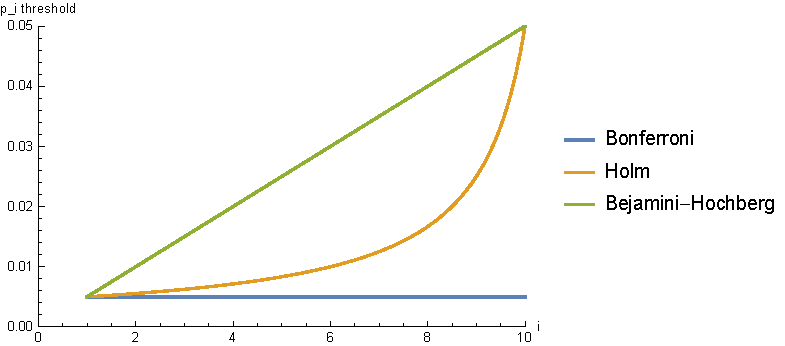
\includegraphics[width=.5\paperwidth]{multiple_testing_plot.pdf}
	\end{figure}
The Bonferroni procedure rejects only the hypotheses under the threshold. The Holm procedure rejects all hypotheses up to the first one that goes above the threshold (even if later hypotheses go below the threshold again). The Benjamini-Hochberg procedure takes the last hypothesis that goes below the threshold and rejects all previous hypotheses (even if some of those are above the threshold).

We see that the Benjamini-Hochberg procedure has more power than the Holm procedure (it rejects more hypotheses). However, since this procedure does not control the FWER, there is less control over type 1 errors. 

Under some assumptions, the Benjamini-Hochberg procedure does control the FDR: 
\begin{theorem}
	Assume that $\qty{p_i \mid i \in I_0}$ are independent, and also independent of $\qty{p_i \mid i \notin I_0}$. Then the Benjamini-Hochberg procedure satisfies
	\[
	\FDR\leq \frac{m_0}{m}\alpha \leq\alpha. 
	\]
\end{theorem}

\begin{remark}
	The independence assumption is quite restrictive: for example, if we have a linear model $Y = X\beta^0 + \eps$ and our hypotheses are $H_i = \qty{\beta_i^0 = 0}$, then all $p_i$ depend on all responses $Y_i$, so in general they will not be independent. In the example sheet we consider a version of the procedure that doesn't require the independence. 
\end{remark}

\begin{proof}
	We have
	\begin{align*}
		\FDR &= \EE\qty[ \frac{N_{01}}{\max(R, 1)}] = \sum_{r=1}^m \EE\qty[\frac{N_{01}}{r} \ind_{R = r}].
	\end{align*}
	Note that when $R = r$, we have by the definition of the procedure that a hypothesis $H_i$ is rejected if and only if $p_i \leq \frac{\alpha r}{m}$.  We therefor continue
	\begin{align*}
		\FDR &= \sum_{r=1}^m \frac 1r \EE\qty[ \sum_{i \in I_0} \ind_{p_i \leq \frac{\alpha r}{m}} \ind_{R = r}]  = \sum_{r=1}^m \frac1r \sum_{i \in I_0} \PP(R = r, p_i \leq \frac{\alpha r}{m}) \\
		&= \sum_{r=1}^m  \frac1r \sum_{i \in I_0} \PP(p_i \leq \frac{\alpha r}{m}) \PP(R = r \mid p_i \leq \frac{\alpha r}{m}) \\
		&\leq \sum_{r=1}^m \frac1r \frac{\alpha r}{m} \sum_{i \in I_0} \PP(R = r \mid P_i \leq \frac{\alpha r}{m})  \\
		&= \frac\alpha m \sum_{i \in I_0} \qty(\sum_{r=1}^m \PP(R = r \mid p_i \leq \frac{\alpha r}{m})) \overset\star= \frac\alpha m \sum_{i \in I_0} 1 = \frac{m_0}{m}\alpha \leq \alpha, 
	\end{align*}
	which proves the claim except that we have to justify $\star$. For this, fix any $i, r$ and let $p^{-i}$ be the set of $p$-values excluding $p_i$ and $p^{-i}_{(1)}, \dotsc, p^{-i}_{(m-1)}$ its order statistics. Note that if $p_i \leq \frac{\alpha r}{m}$ and $R = r$, then $p_i \in \qty{p_{(1)}, \dotsc, p_{(m)}}$, so we have
	\begin{align*}
		\PP(R = r \mid p_i \leq \frac{\alpha r}{m}) &= \PP(p_{(r)} \leq \frac{\alpha r}{m}, p_{(s)} > \frac{\alpha s}{m} \ \forall s > r \mid p_i \leq \frac{\alpha r}{m}) \\
		&= \PP(p^{-i}_{(r-1)} \leq \frac{\alpha r}{m}, p^{-i}_{(s-1)} > \frac{\alpha s}{r} \ \forall s > r \mid p_i \leq \frac{\alpha r }{m}) \\
		&= \PP(p^{-i}_{(r-1)} \leq \frac{\alpha r}{m}, p^{-i}_{(s-1)} > \frac{\alpha s}{r} \ \forall s > r) &\text{(by independence)} \\
		&= \PP(\max \qty{1 \leq \ell \leq m : p_{(\ell -1 )}^{-i} \leq \frac{\alpha \ell}{m}} = r) \\
		&\eqqcolon \PP(Z = r),
	\end{align*}
	where we define $p_{(0)}^{-i} \ceq 0$. Noting that $Z$ takes values in $\qty{1, \dotsc, m}$, we have
	\[
	\sum_{r=1}^m \PP(R = r \mid p_i \leq \frac{\alpha r}{m}) = \sum_{r = 1}^m \PP(Z =r) = 1,
	\]
	which concludes the proof.
\end{proof}
\end{example}

\subsection{Inference in high-dimensional regression}
Recall that with \emph{inference} we mean the forming of confidence intervals and the testing of hypotheses. We consider our usual model $Y = X\beta^0 + \eps$ where $\eps \sim \Rm N(0, \sigma^2 I)$. 

In the classical situation $n \gg p$, it is known that $\hat\beta^\Rm{OLS} - \beta^0 \sim \Rm N(0, \sigma^2 (X\T X)^{-1})$, and therefore we obtain the ellipsoidal confidence set
\[
\qty{\beta : \frac{\norm{\beta - \hat\beta^\Rm{OLS}}_2^2}{p\hat\sigma^2} \leq t}
\]
where $\hat\sigma$ is an unbiased estimator of $\sigma$, and this confidence set contains the true parameter with probability $\PP(Z \leq t)$, where $Z \sim F_{p, n-p}$. We can use this to test hypotheses such as $H: \beta_j^0 = 0$.

However, when $p  \gg n$, even when $\beta^0$ is assumed to be sparse it is much harder to obtain confidence sets, because the distribution of $\hat\beta_\lambda^L - \beta^0$  is difficult to characterise as there is no explicit formula for $\hat\beta_\lambda^L$. 
Specifically, the dependence on $\beta^0$ and $X$ is nontrivial.  

One option is to consider the \emph{debiased Lasso estimator}. 
We start with the KKT conditions (writing $\hat S = \qty{k : \hat\beta_k \neq 0}$): 
\[
\frac1n X\T (Y - X\hat\beta) = \lambda\hat\nu, \quad \norm{\hat\nu}_\infty \leq 1, \quad \hat\nu_{\hat S} = \sign(\hat\beta_{\hat S}). 
\]
Write $\hat\Sigma = X\T X / n$, then we can rewrite the conditions as
\begin{align*}
	\frac1n X\T (X(\beta^0 + \eps) - X\hat\beta) &= \lambda\hat\nu \\
	\hat\Sigma(\beta^0 - \hat\beta) + \frac1nX\T\eps &= \lambda\hat\nu \\
	\hat\Sigma(\hat\beta - \beta^0) + \lambda\hat\nu &= \frac1nX\T \eps. 
\end{align*}
Suppose now that $\hat\Theta$ is an approximate inverse of $\hat\Sigma$ (which we will not yet define, but it must be the case that $\hat\Theta\hat\Sigma - I$ is small in some sense). Multiplying by the left with $\hat\Theta$ we obtain
\begin{align*}
	\hat\Theta\hat\Sigma (\hat\beta - \beta^0) + \lambda\hat\Theta \hat\nu &= \frac1n \hat\Theta X\T\eps \\
	\hat\beta - \beta^0 + (\hat\Theta\hat\Sigma - I)(\hat\beta - \beta^0) + \lambda\hat\Theta\hat\nu &= \frac1n \hat\Theta X\T \eps \\
	\hat\beta + \lambda\hat\Theta\hat\nu - \beta^0 &= \frac1n \hat\Theta X\T \eps + (\hat\Theta\hat\Sigma - I)(\beta^0 - \hat\beta) \\
	\hat\beta + \lambda\hat\Theta\hat\nu - \beta^0 &= \frac1n \hat\Theta X\T\eps + \frac1{\sqrt n} \Delta, 
\end{align*}
where $\Delta \ceq \sqrt n(\hat\Theta\hat\Sigma - I)(\beta^0 - \hat\beta)$. Considering this expression, we can define the \emph{debiased Lasso estimator} by
\[
\hat b \ceq \hat\beta + \lambda \hat\Theta \hat\nu  = \hat\beta  + \Theta X\T (Y - X\hat\beta) / n, 
\]
and the above expression becomes
\begin{equation}\label{eq:debiased_lasso_error}
	\hat b - \beta^0 = \frac1n \hat\Theta X\T\eps + \frac1{\sqrt n} \Delta. 
\end{equation}
This allows us to almost understand the distribution of $\hat b - \beta^0$: we know that $\frac1n \hat\Theta X\T\eps$ is normally distributed, while for an appropriate choice of $\hat\Theta$, the vector $\Delta$ can be made small. 

For a matrix $A$, let $A_{j, \cdot}$ denote its $j$th row. We then have
\begin{align*}
	\norm{\Delta}_\infty &= \sqrt n\max_j \abs{(\hat\Theta\hat\Sigma - I)_{j, \cdot}\T (\hat\beta - \beta^0)} \\
	&\leq  \sqrt n \qty(\max_j \norm{(\hat \Theta\hat\Sigma - I)_{j, \cdot}}_\infty)\norm{\hat\beta - \beta^0}_1. 
\end{align*}
We already have bounds on $\norm{\hat\beta - \beta^0}_1$ using either \cref{thm:lasso_slow_rate} or \cref{thm:lasso_fast_rate}. Therefore we focus on the rows of $\hat\Theta\hat\Sigma - I$. Letting $\hat\theta_j \ceq \Theta_{j, \cdot}$, we have for any $\eta \geq 0$ that 
\begin{align}
	\norm{(\hat\Theta\hat\Sigma - I)_{j, \cdot}}_\infty \leq \eta &\iff 
		\abs{(\hat\Theta\hat\Sigma)_{j, j} - 1} \leq \eta \text{ and for $i \neq j$: } \abs{(\hat\Theta\hat\Sigma)_{j, i}} \leq \eta \nonumber \\
		&\iff \abs{X_j\T X \hat\theta_j / n - 1} \leq \eta  \text{ and } \frac1n\norm{X_{-j}\T X \hat\theta_j}_\infty \leq \eta \label{eq:debiased_lasso_bound_conds}
\end{align}
where $X_{-j}$ is the matrix $X$ with the $j$th column excluded. Note that the first inequality concerns the diagonal elements of $\hat\Theta\hat\Sigma$ while the second concerns the off-diagonal elements. 

We define
\begin{equation} \label{eq:lasso_regress_column}
\hat\gamma^{(j)} \ceq \argmin_{\gamma \in \RR^{p-1}} \qty{\frac1{2n} \norm{X_j - X_{-j}\gamma}_2^2 + \lambda_j \norm{\gamma}_1}, 
\end{equation}
which is the lasso estimator for regressing $X_j$ onto $X_{-j}$ where $\lambda_j$ is some tuning parameter. Furthermore, we define 
\[
\hat\tau_j^2 = \frac1n \norm{X_j - X_{-j}\hat\gamma^{(j)}}_2^2 + \lambda_j \norm{\gamma^{(j)}}_1 \overset{\Rm{ES}}=  X_j\T (X_j - X_{-j}\hat\gamma^{(j)})/n. 
\]
We now define the matrix $\hat\Theta$ by setting its rows has
\[
\hat\theta_j = - \frac{1}{\hat \tau_j^2} (\hat \gamma_1^{(j)}, \dotsc, \hat\gamma_{j-1}^{(j)}, -1, \hat\gamma_j^{(j)}, \dotsc, \hat\gamma_{p-1}^{(j)})\T  \in \RR^p, 
\]
so that
\[
X\hat\theta_j = -\frac{1}{\hat\tau_j^2} \qty(X_{-j}\hat\gamma^{(j)}  - X_j) = \frac{X_j - X_{-j}\gamma^{(j)}}{X_j\T (X_j - X_{-j}\gamma^{(j)}) / n}. 
\]

We now consider the conditions from \cref{eq:debiased_lasso_bound_conds}.  For the first one, note that $X_j\T X \hat\theta_j / n = 1$, so that conditions is satisfied for any $\eta$. For the second one, letting $\tilde\nu^{(j)}$ denote the vector appearing in the KKT conditions for $\hat\gamma^{(j)}$ (\cref{eq:lasso_regress_column}), we have that
\[
\frac1n X_{-j}\T(X \hat\theta_j) = \frac1{n\hat\tau_j^2} X_{-j}\T (X_j - X_{-j}\hat\gamma^{(j)}) = \frac{\lambda_j \tilde \nu^{(j)}}{\hat\tau_j^2} \implies \frac1n \norm{X_{-j}\T X \hat\theta_j}_\infty \leq \frac{\lambda_j}{\hat\tau_j^2}. 
\]
Note that $\lambda_j$ and $\hat\tau_j$ do not depend on the responses $Y$ for our original problem in any way.  Putting everything together, we find
\[
\norm{\Delta}_\infty\leq \sqrt n \norm{\hat\beta - \beta^0}_1 \cdot \max_j \frac{\lambda_j}{\hat\tau_j^2}.
\]

Therefore, we must only understand how we can make $\lambda_j/\hat\tau_j^2$ small. First we will briefly consider its practical use. 

\subsubsection{Using the debiased Lasso in practice}
Under the assumption that $\norm{\Delta}_\infty$ is small, we have by \cref{eq:debiased_lasso_error} that
\[
\sqrt n(\hat b_j  - \beta^0_j) \approx  W_j, 
\]
where $W_j = (\frac1n \hat\Theta X\T\eps)_j \sim \Rm N(0, \sigma^2 (\hat\Theta\hat\Sigma\hat\Theta\T)_{jj}) \eqqcolon \Rm N(0, \sigma^2 d_j)$.

Therefore, an \emph{approximate} $(1 - \alpha)$-level confidence interval for $\beta^0_j$ is given by 
\[
\qty[\hat b_j - z_{\alpha/2} \sigma \sqrt{d_j/n} , \hat b_j + z_{\alpha / 2} \sigma \sqrt{{d_j}/{n}}],
\]  
(\TODO Recap how to construct confidence intervals).  The only unknown in the above expression is $\sigma$, which must be estimated. 
